% Supplementary / Extended Data Figures for Sun et al. 2020
% Chapter: Hippocampal neurons represent events as transferable units of experience

\section*{Extended Data Figures}

\begin{figure}[htbp]
\centering
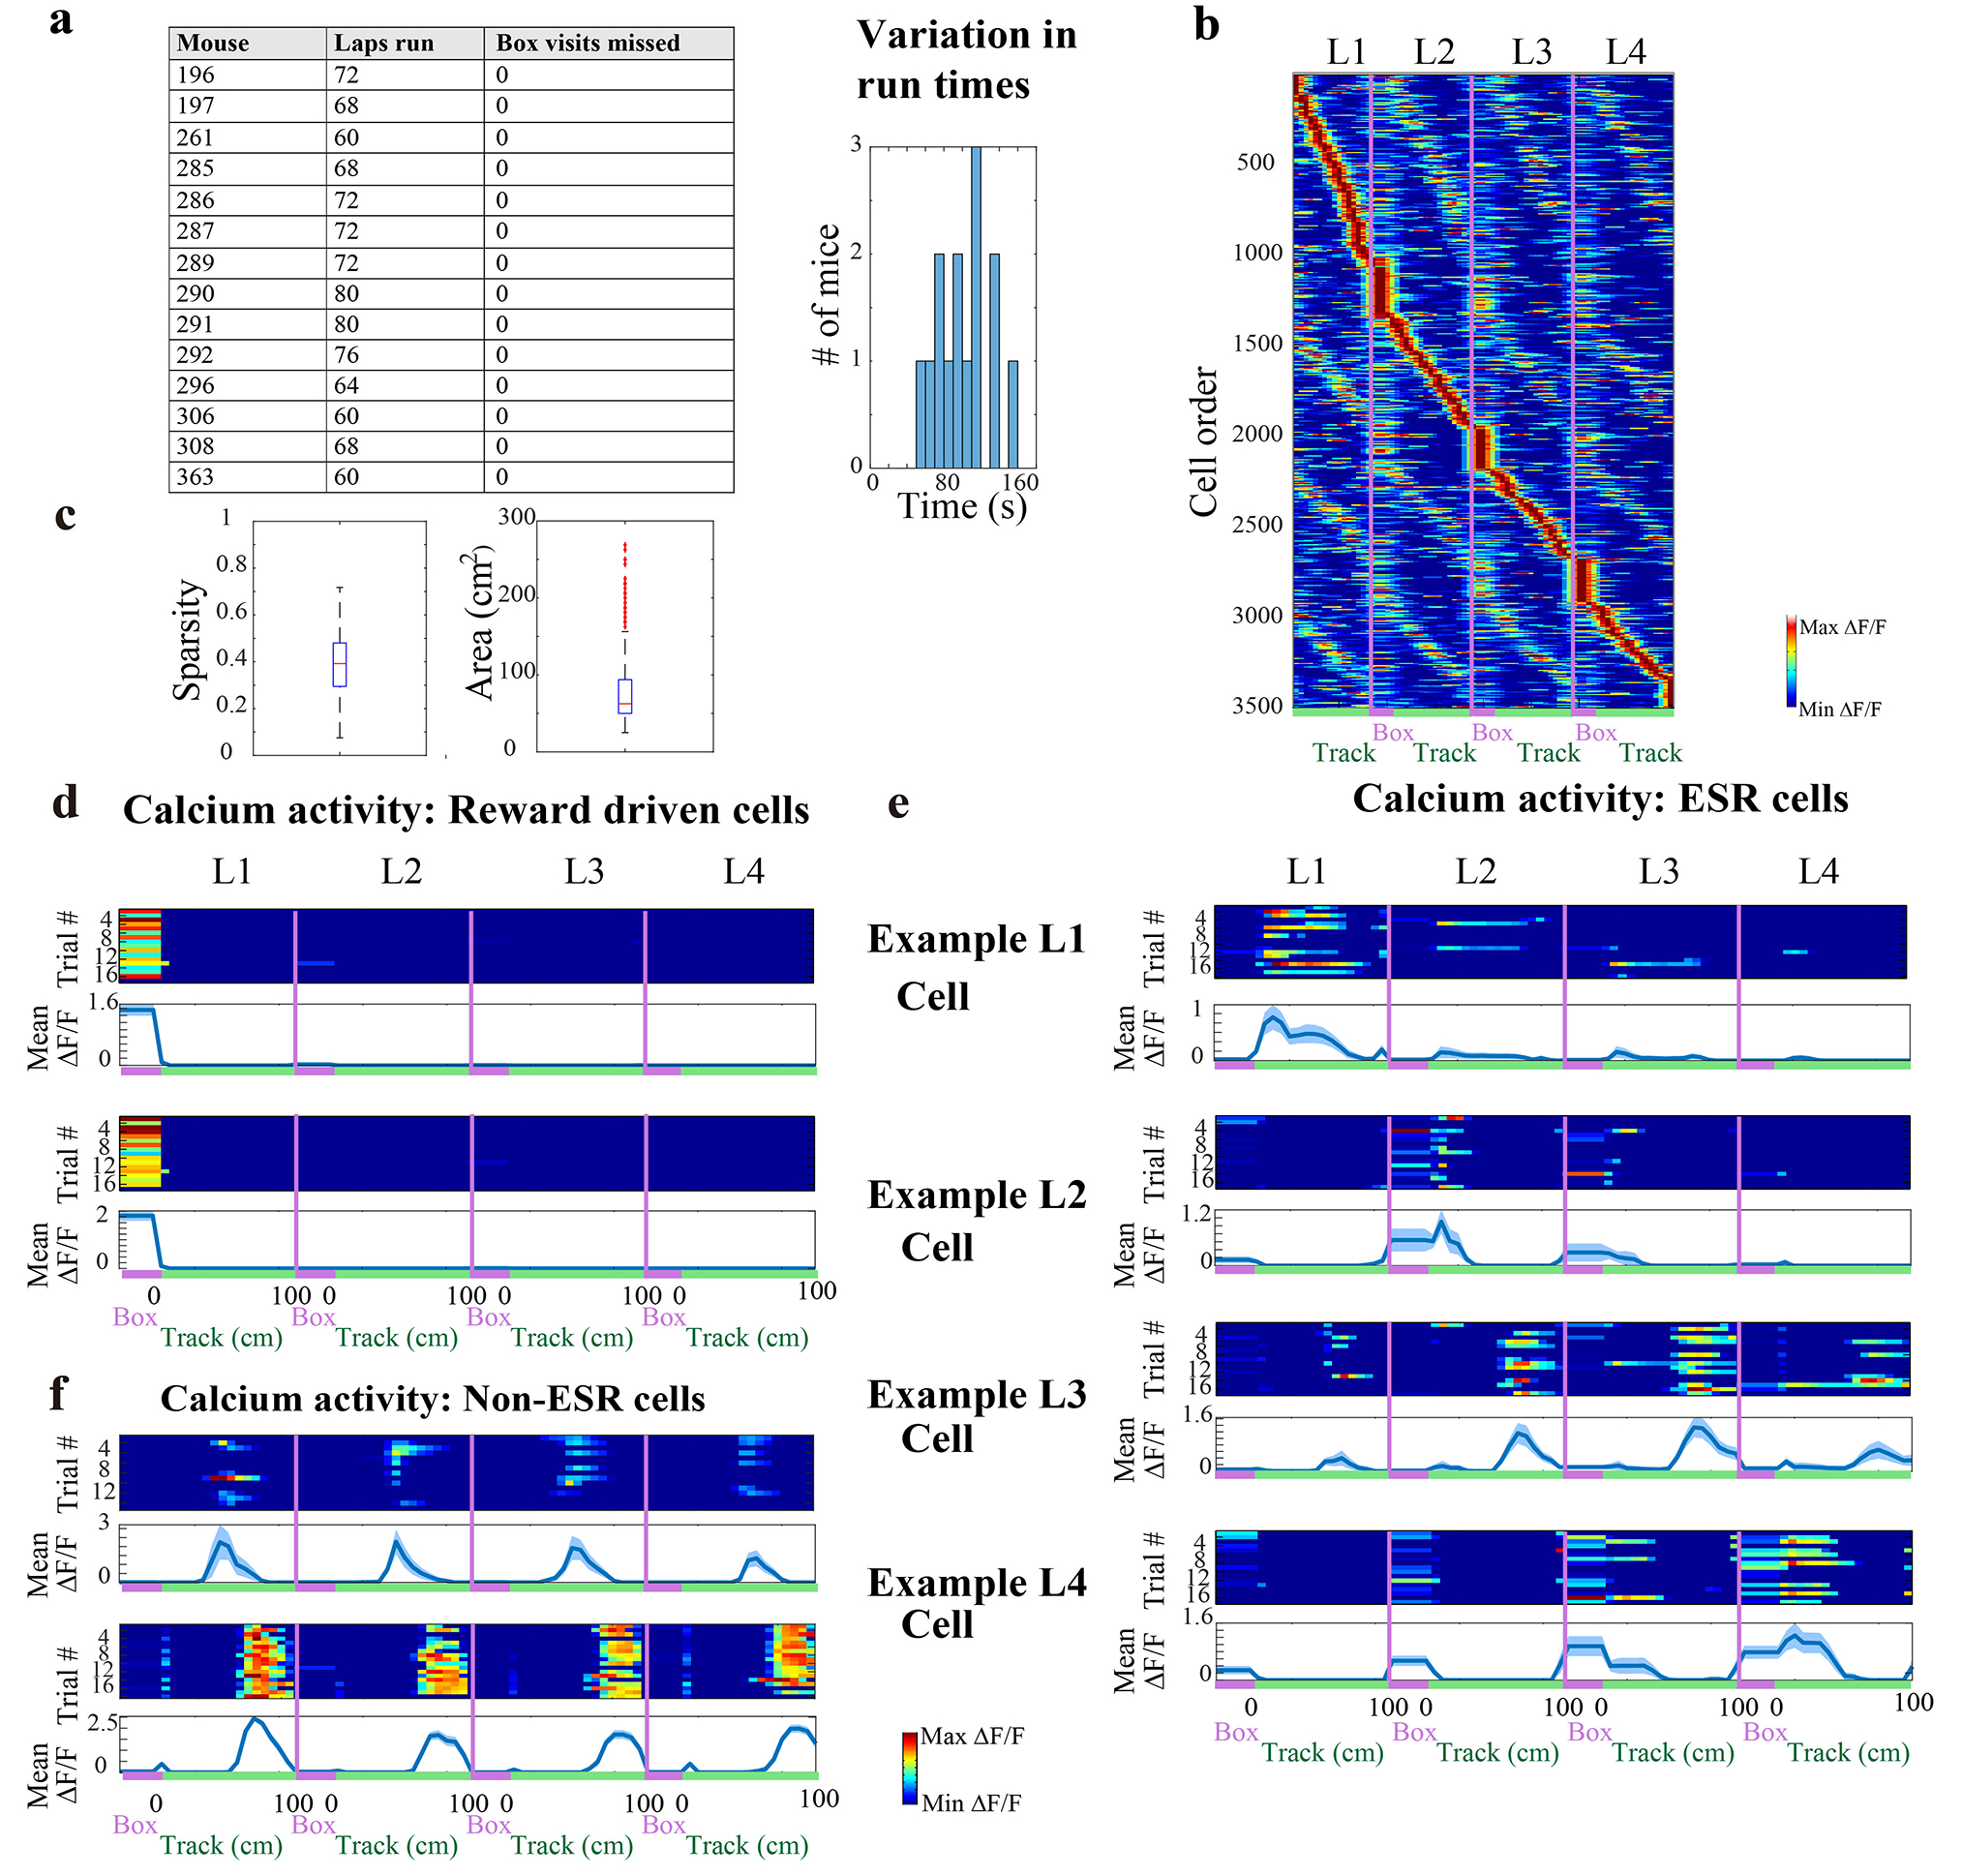
\includegraphics[width=\textwidth]{figures/ch_sun2020/extended_fig1.jpg}
\caption[Extended Data Fig.~1: Behavioral and imaging characterization]{\textbf{Extended Data Fig.\ 1: Behavioral and imaging characterization.}
(a) Left: reward box visit behavior across laps, confirming animals visited the reward box after every lap regardless of reward delivery. Right: trial duration distributions.
(b) Rate remapping of ESR cells in the standard 4-lap task, illustrated in raw $\Delta F/F$ activity at the peak spatial bin.
(c) Spatial selectivity of CA1 neurons recorded during the square maze task.
(d) Examples of reward-driven cells active during reward consumption (lap 1 in the reward box); these cells were excluded from further ESR analysis.
(e) Trial-by-trial calcium activity illustrating the stochastic yet lap-specific nature of ESR cell activation across trials.}
\label{fig:sun2020-ext1}
\end{figure}

\begin{figure}[htbp]
\centering
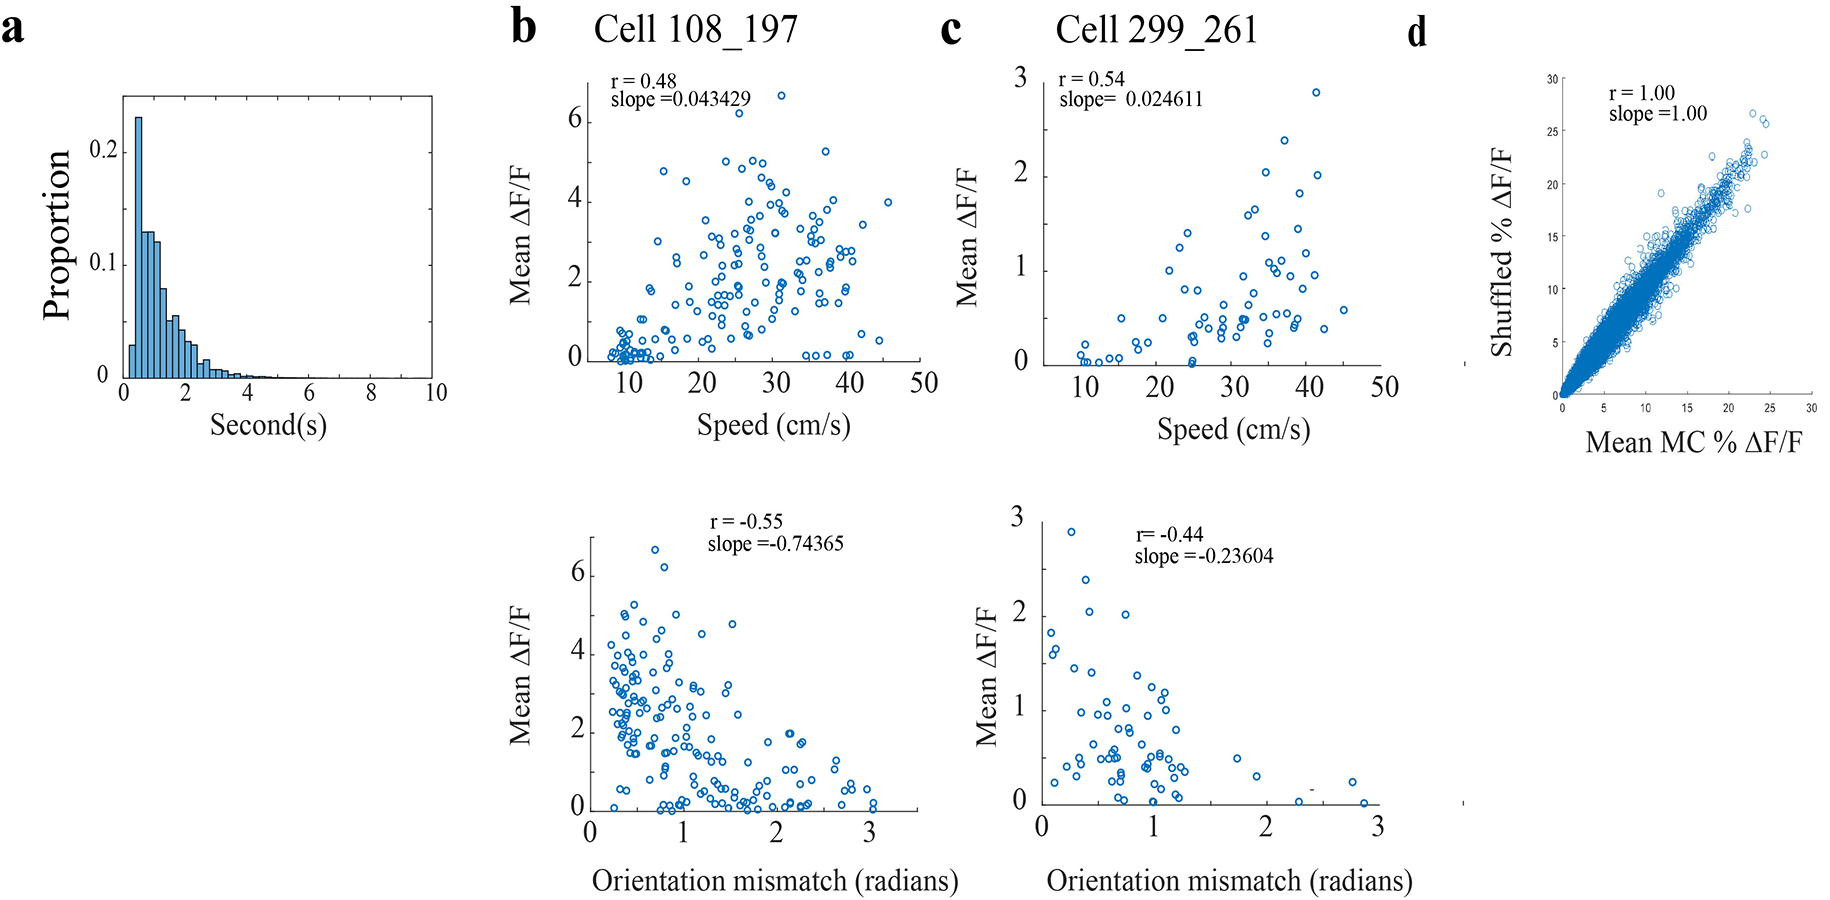
\includegraphics[width=\textwidth]{figures/ch_sun2020/extended_fig2.jpg}
\caption[Extended Data Fig.~2: Calcium transient characteristics and model validation]{\textbf{Extended Data Fig.\ 2: Calcium transient characteristics and model validation.}
(a) Distribution of calcium transient decay times across $n=14$ animals (137,045 calcium events; median decay time $= 1.35$\,s).
(b) Speed tuning of CA1 neurons: relationship between mean running speed and calcium activity, used in the linear model for ESR cell identification.
(c) Head direction tuning of CA1 neurons: relationship between head orientation and calcium activity.
(d) Shuffled calcium activity level distributions confirming the validity of the linear model used for model correction.}
\label{fig:sun2020-ext2}
\end{figure}

\begin{figure}[htbp]
\centering
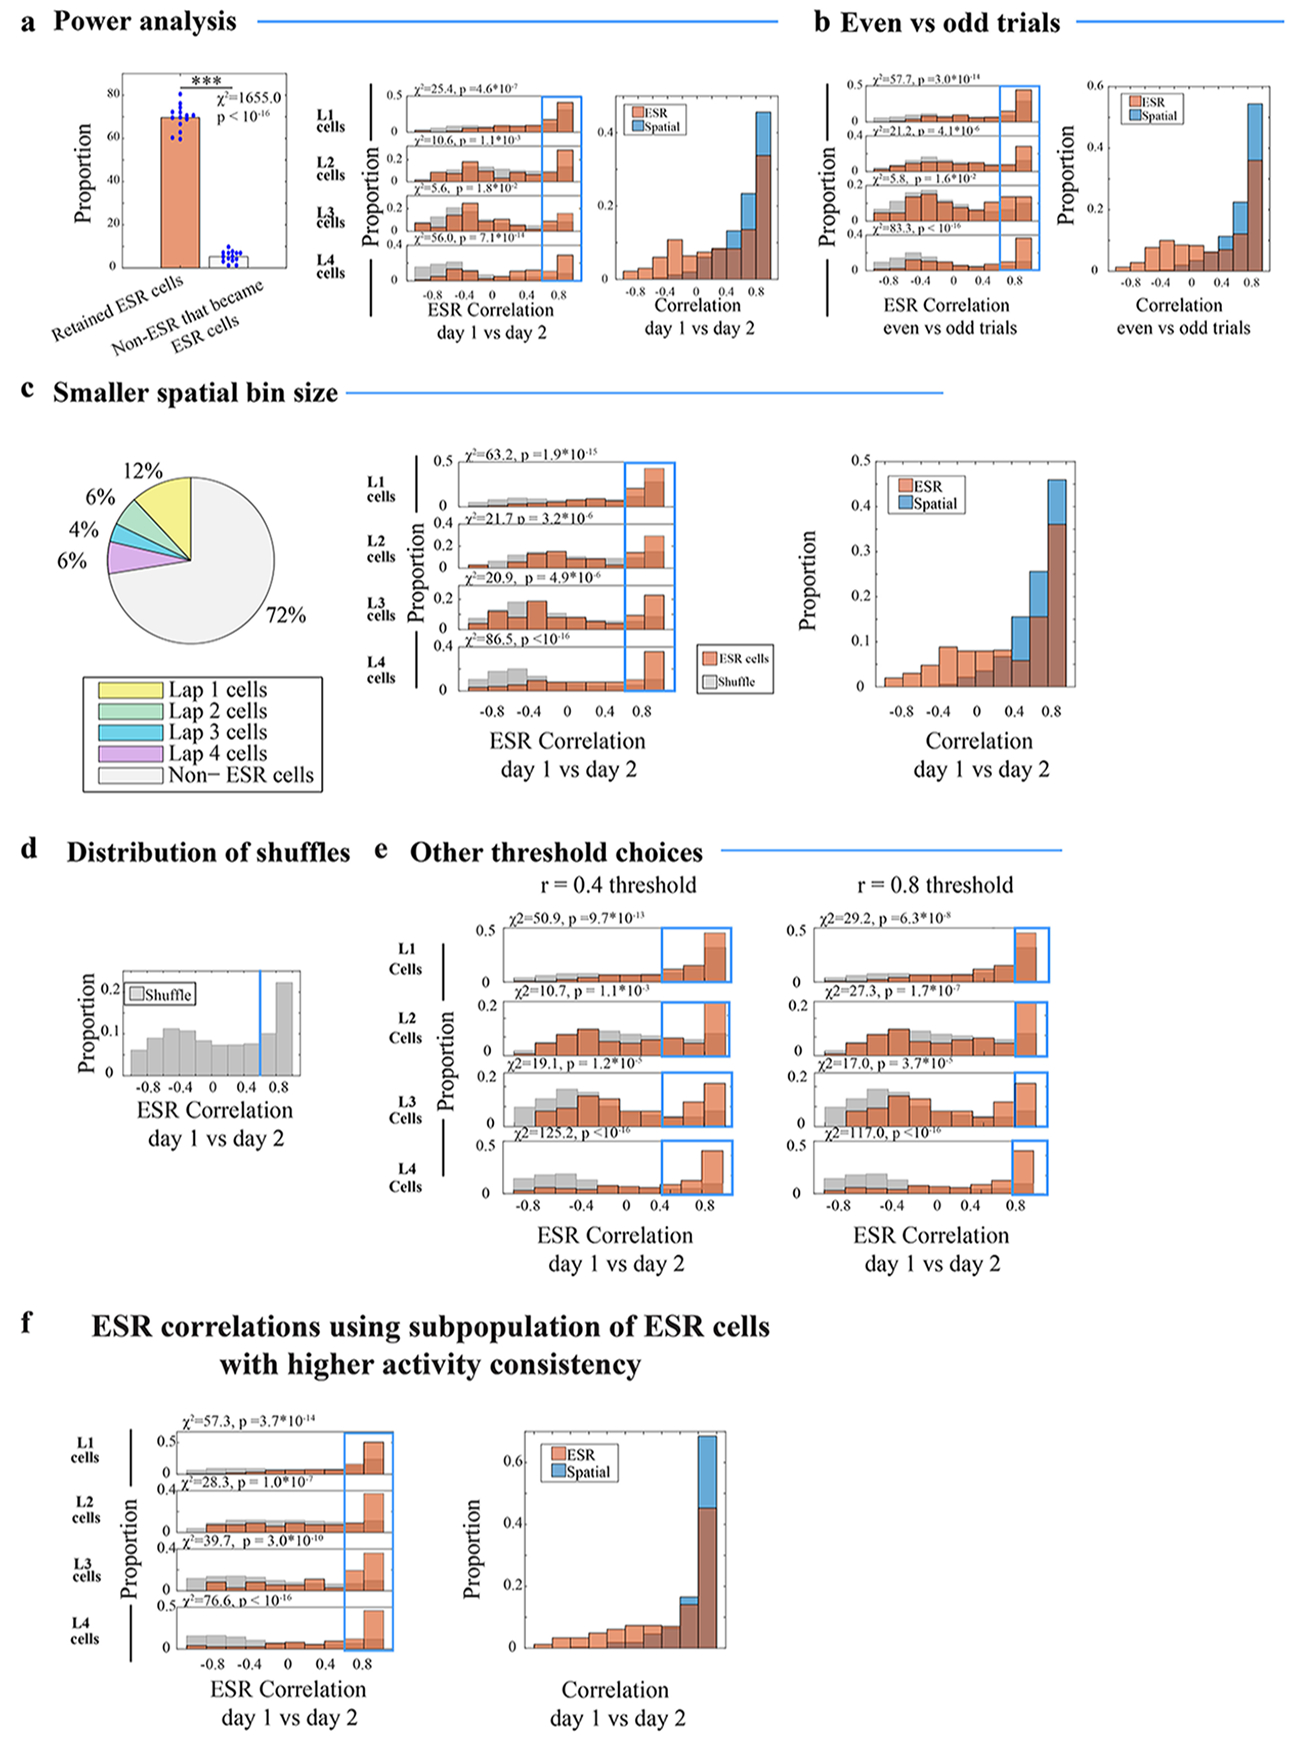
\includegraphics[width=\textwidth]{figures/ch_sun2020/extended_fig3.jpg}
\caption[Extended Data Fig.~3: ESR cell stability across conditions]{\textbf{Extended Data Fig.\ 3: ESR cell stability across conditions.}
(a) Additional example ESR cells illustrating lap-specific activity patterns in the standard 4-lap-per-trial task.
(b) ESR cell percentages across sessions confirming that the proportion of lap-modulated cells is consistent across repeated testing days within individual animals.}
\label{fig:sun2020-ext3}
\end{figure}

\begin{figure}[htbp]
\centering
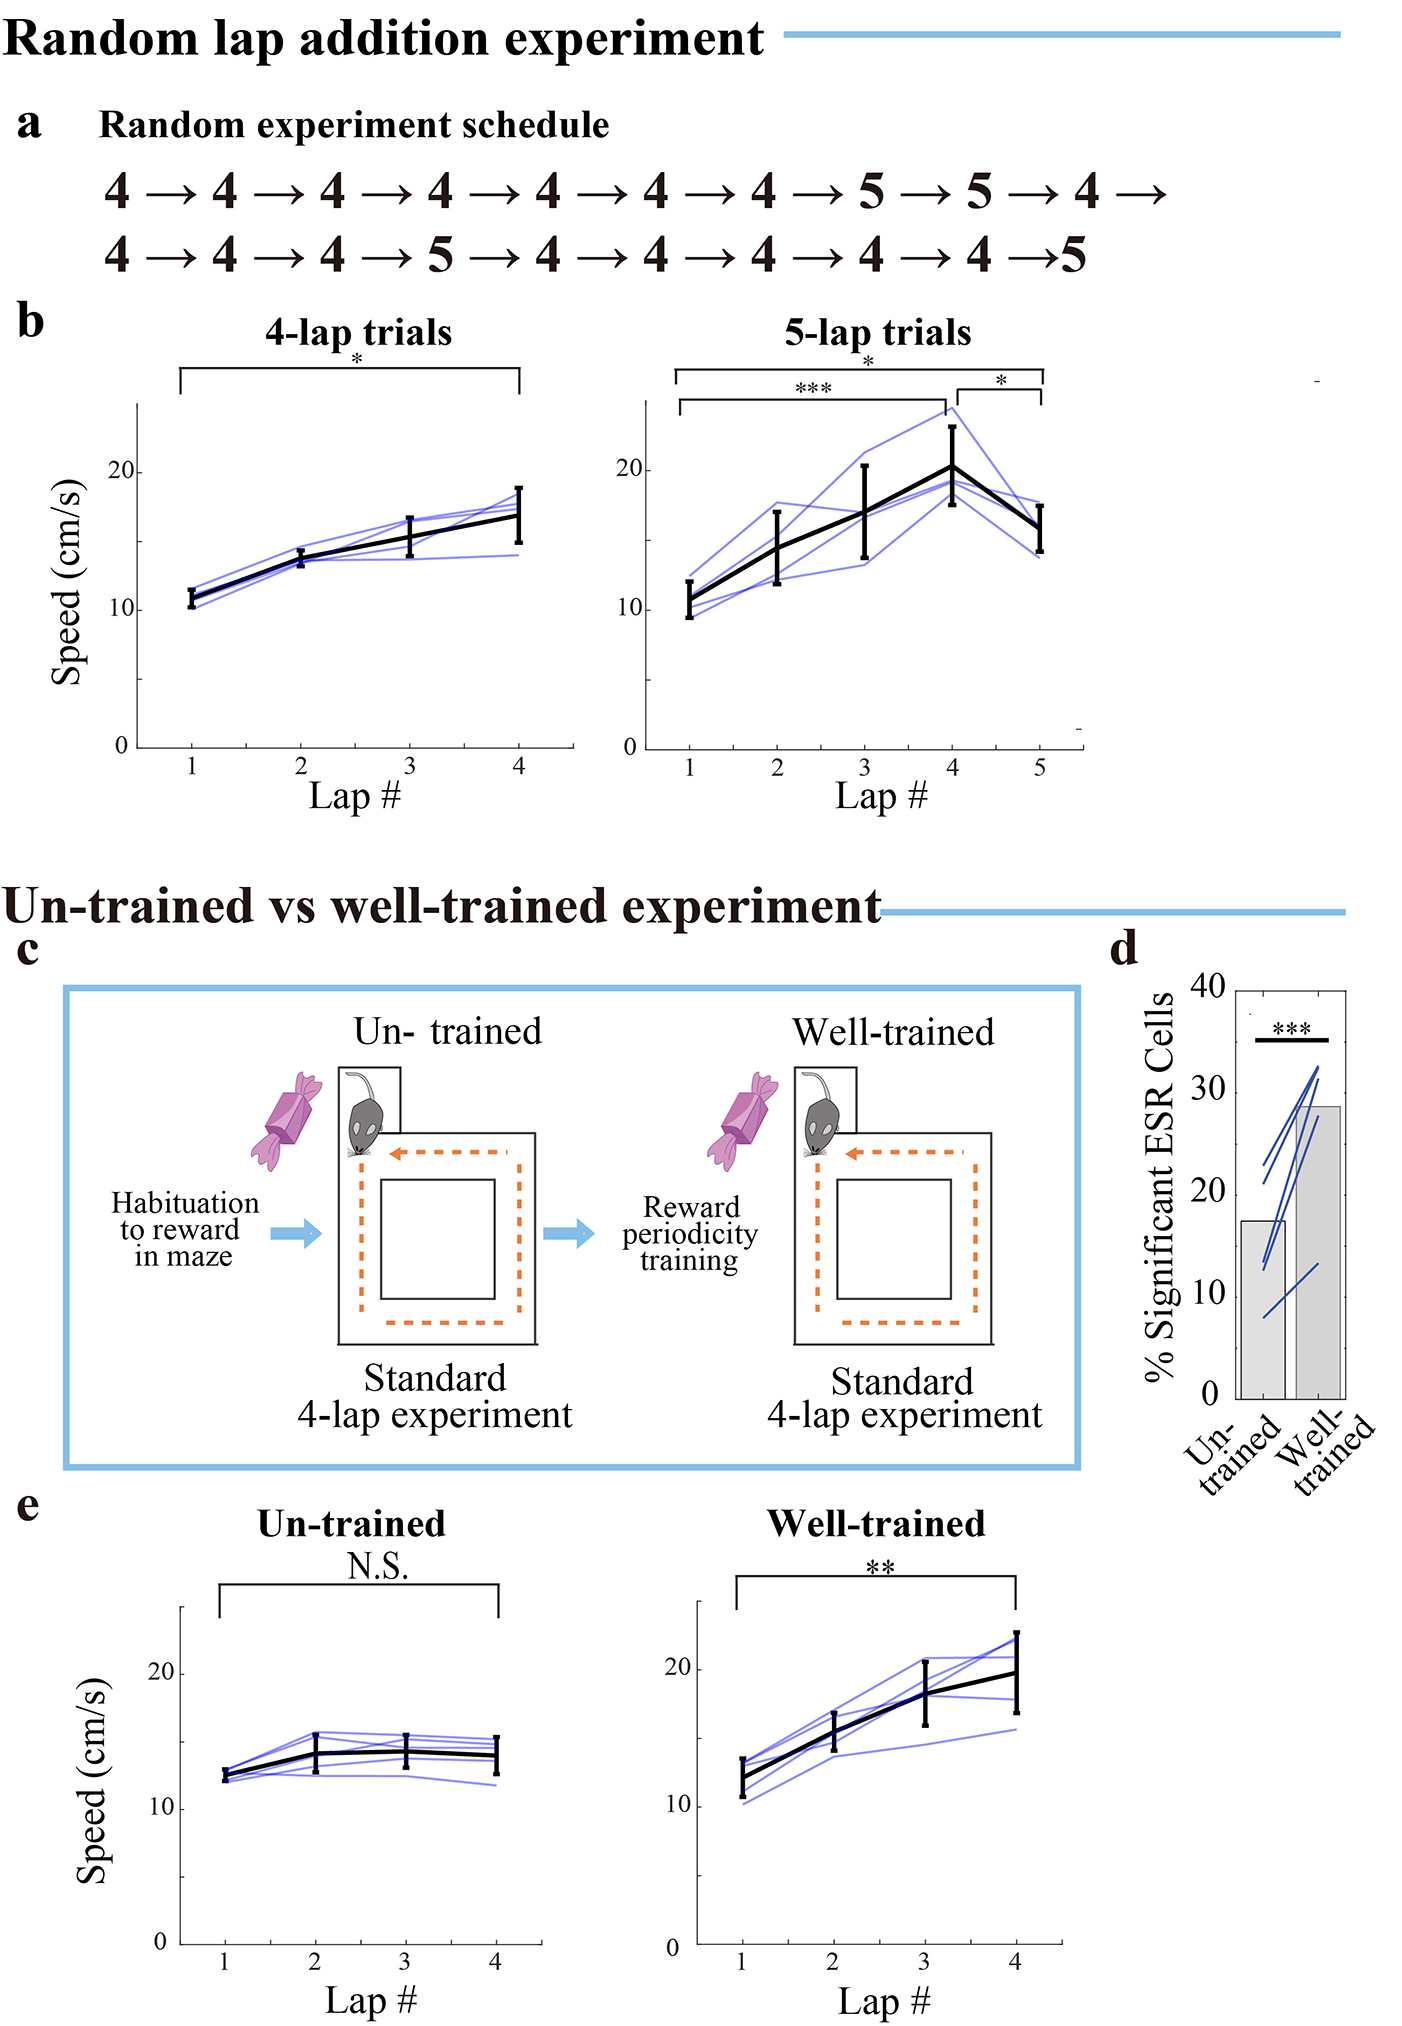
\includegraphics[width=\textwidth]{figures/ch_sun2020/extended_fig4.jpg}
\caption[Extended Data Fig.~4: Learning of ESR activity patterns]{\textbf{Extended Data Fig.\ 4: Learning of ESR activity patterns.}
(a) Behavioral data confirming that well-trained animals ran significantly faster during lap 4 compared to lap 1.
(b) Reward anticipation behavior: when reward was unexpectedly delayed by one lap, animals ran significantly slower during the extra 5th lap compared to lap 4.
(c--d) ESR cell percentages for na\"{i}ve animals (first exposure to the 4-lap task, 17\% = 176/1008 cells, $n=5$ mice) vs.\ well-trained animals (29\% = 335/1168 cells; $\chi^2=37.9$, $p=7.4 \times 10^{-10}$).
(e) ESR activity patterns across days for the na\"{i}ve vs.\ trained comparison.}
\label{fig:sun2020-ext4}
\end{figure}

\begin{figure}[htbp]
\centering
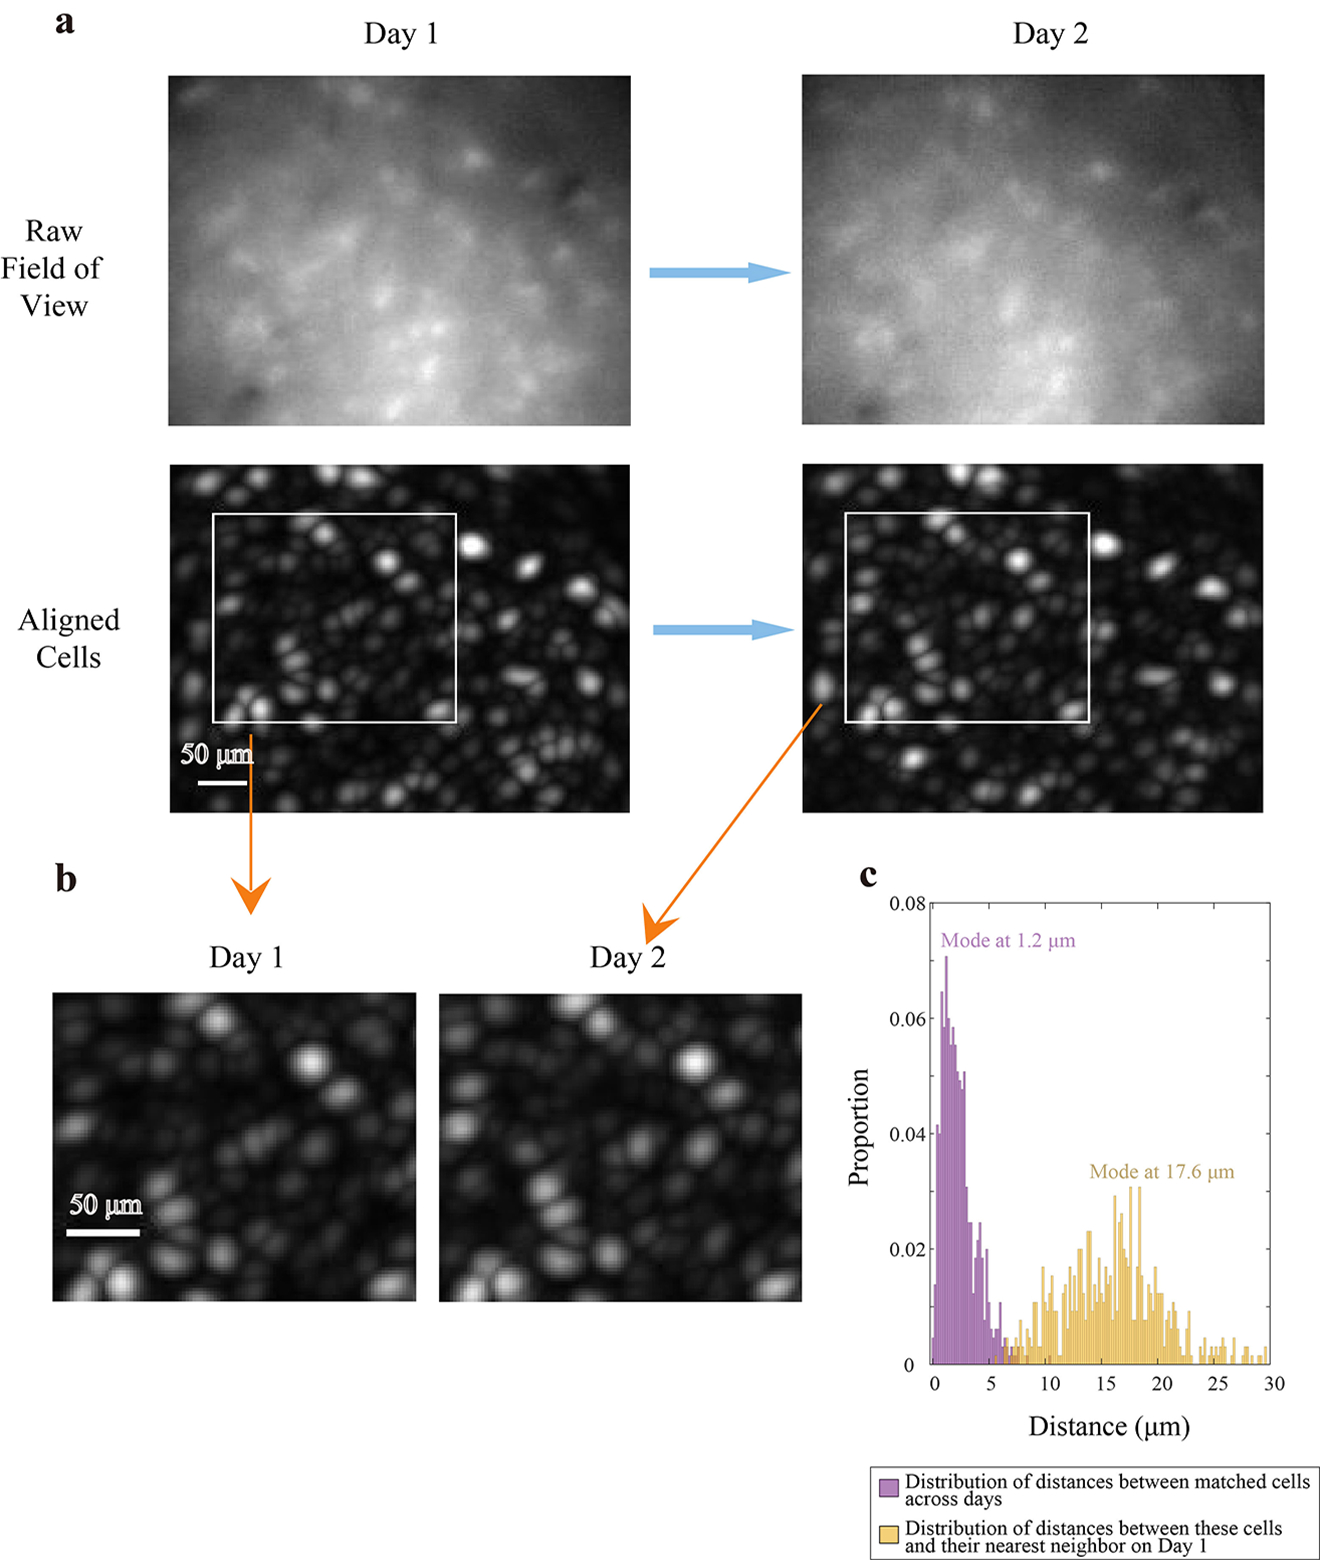
\includegraphics[width=\textwidth]{figures/ch_sun2020/extended_fig5.jpg}
\caption[Extended Data Fig.~5: Cell tracking across days]{\textbf{Extended Data Fig.\ 5: Cell tracking across days.}
Cell registration approach used to match individual ESR cells across consecutive imaging days, confirming that the same physical neurons were tracked when computing cross-day ESR correlations.}
\label{fig:sun2020-ext5}
\end{figure}

\begin{figure}[htbp]
\centering
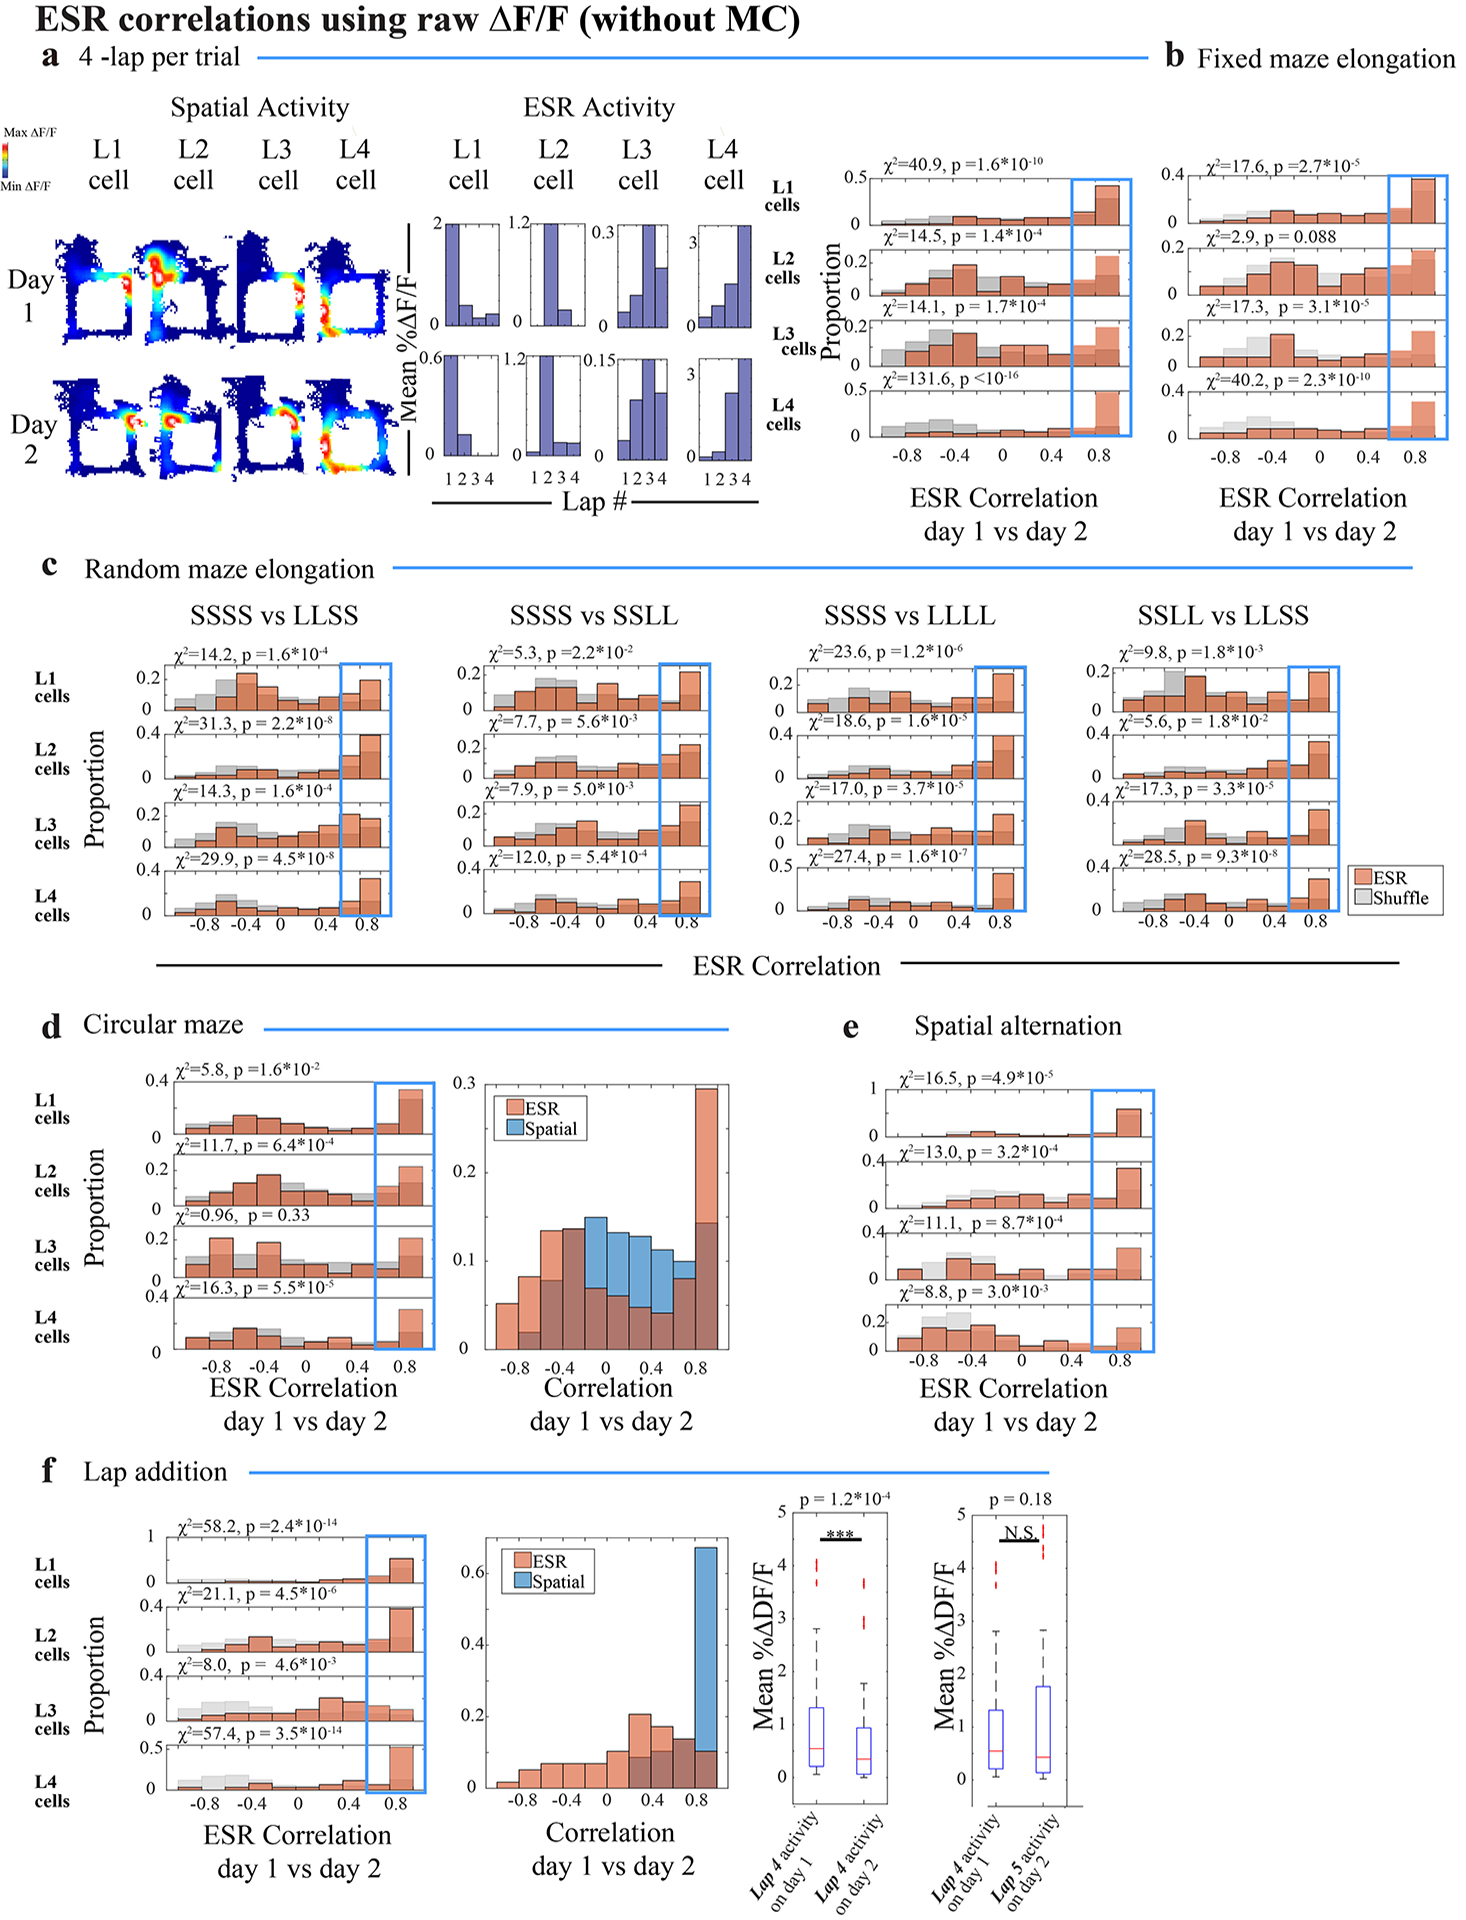
\includegraphics[width=\textwidth]{figures/ch_sun2020/extended_fig6.jpg}
\caption[Extended Data Fig.~6: Raw $\Delta F/F$ results without model correction]{\textbf{Extended Data Fig.\ 6: Raw $\Delta F/F$ results without model correction.}
Analogous to the model-corrected (MC) results reported in the main figures, raw $\Delta F/F$ ESR correlations are shown for each major experiment: (a) standard 2-day experiment, (b) fixed maze elongation, (c) random maze elongation, (d) circular maze, (e) spatial alternation, and (f) lap addition experiment. Results are consistent with model-corrected analyses, confirming that the ESR phenomenon is not an artifact of the linear model subtraction procedure.}
\label{fig:sun2020-ext6}
\end{figure}

\begin{figure}[htbp]
\centering
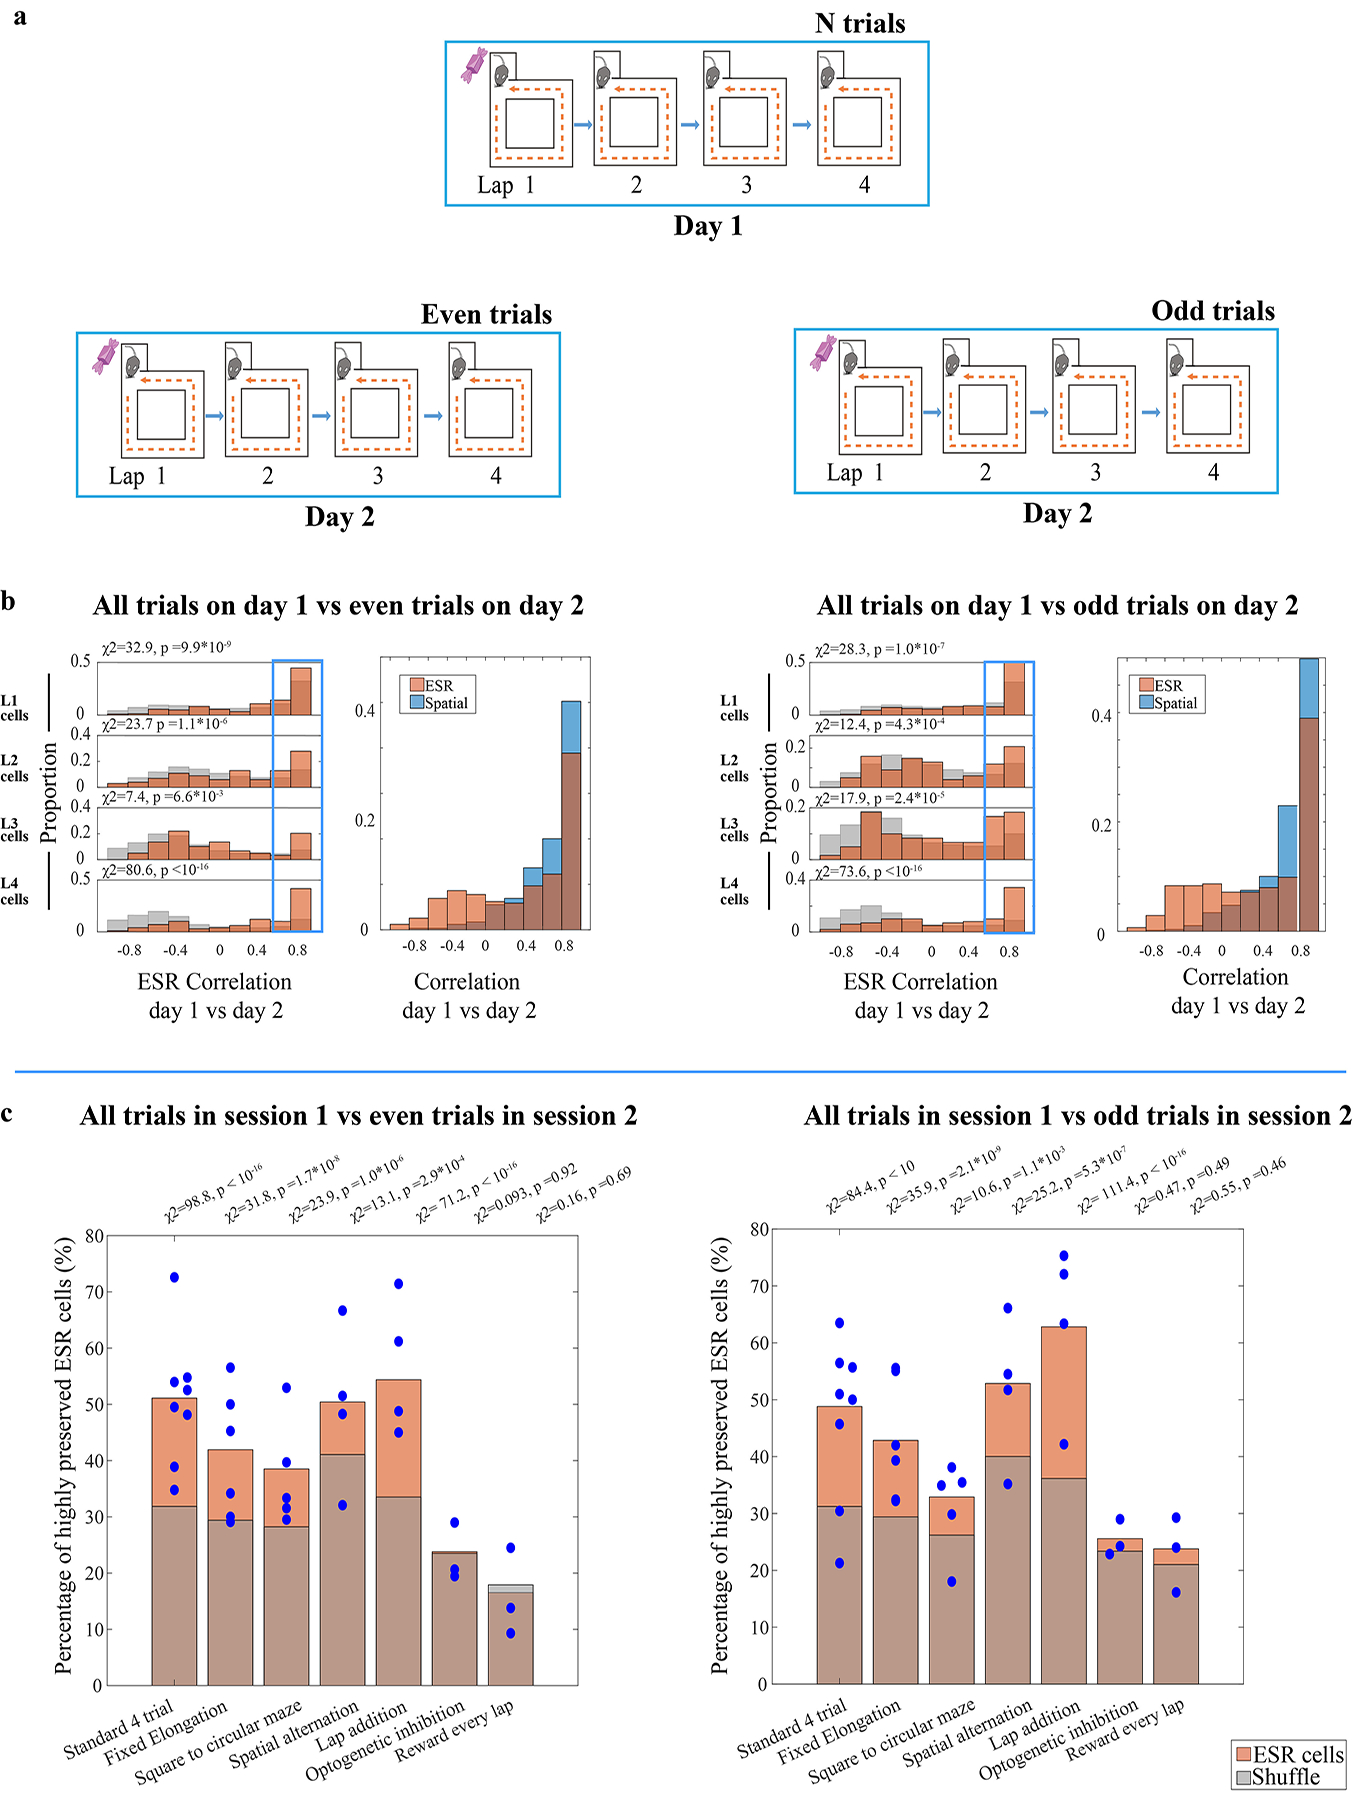
\includegraphics[width=\textwidth]{figures/ch_sun2020/extended_fig7.jpg}
\caption[Extended Data Fig.~7: ESR preservation with reduced trial subsampling]{\textbf{Extended Data Fig.\ 7: ESR preservation with reduced trial subsampling.}
(a--c) ESR correlations computed when half the trials are randomly eliminated, demonstrating that lap-specific activity patterns are robustly preserved even with substantially reduced data. This rules out the possibility that ESR preservation simply reflects over-fitting to a large number of trials.}
\label{fig:sun2020-ext7}
\end{figure}

\begin{figure}[htbp]
\centering
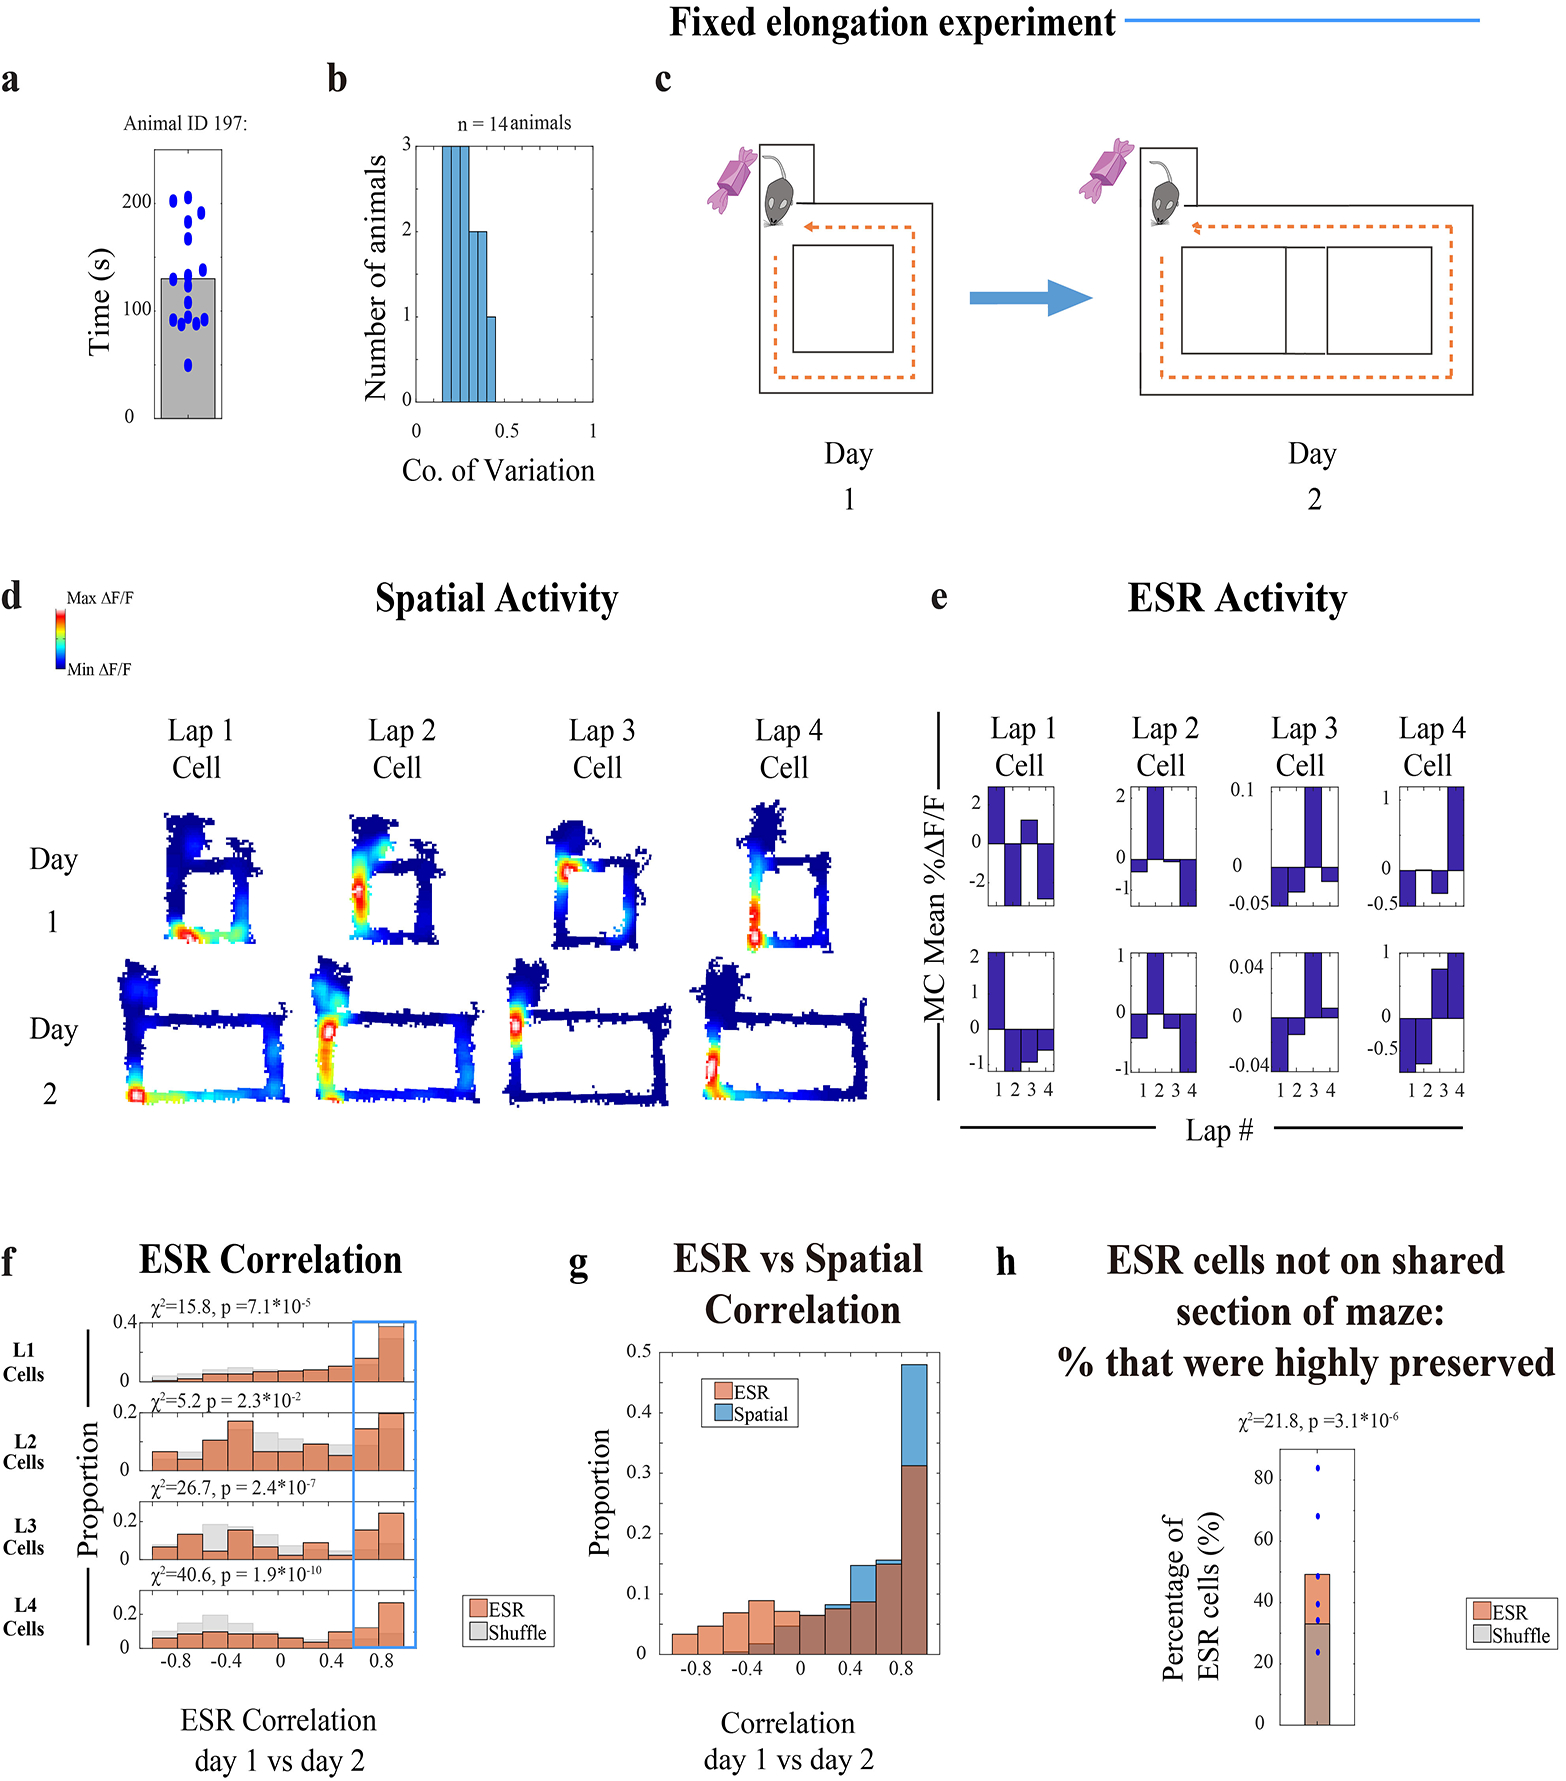
\includegraphics[width=\textwidth]{figures/ch_sun2020/extended_fig8.jpg}
\caption[Extended Data Fig.~8: Fixed maze elongation experiment]{\textbf{Extended Data Fig.\ 8: Fixed maze elongation experiment.}
(a--b) Distributions of trial durations and running speeds, confirming that animals ran at varying speeds and took unpredictable and variable times to complete laps.
(c) Fixed maze elongation experiment design: the maze was elongated in one dimension to twice the standard length.
(d--e) Example cells with preserved ESR activity patterns across standard and elongated maze sessions.
(f) ESR correlations across standard vs.\ elongated maze sessions, confirming that ESR activity tracks lap events rather than total continuous distance traveled.}
\label{fig:sun2020-ext8}
\end{figure}

\begin{figure}[htbp]
\centering
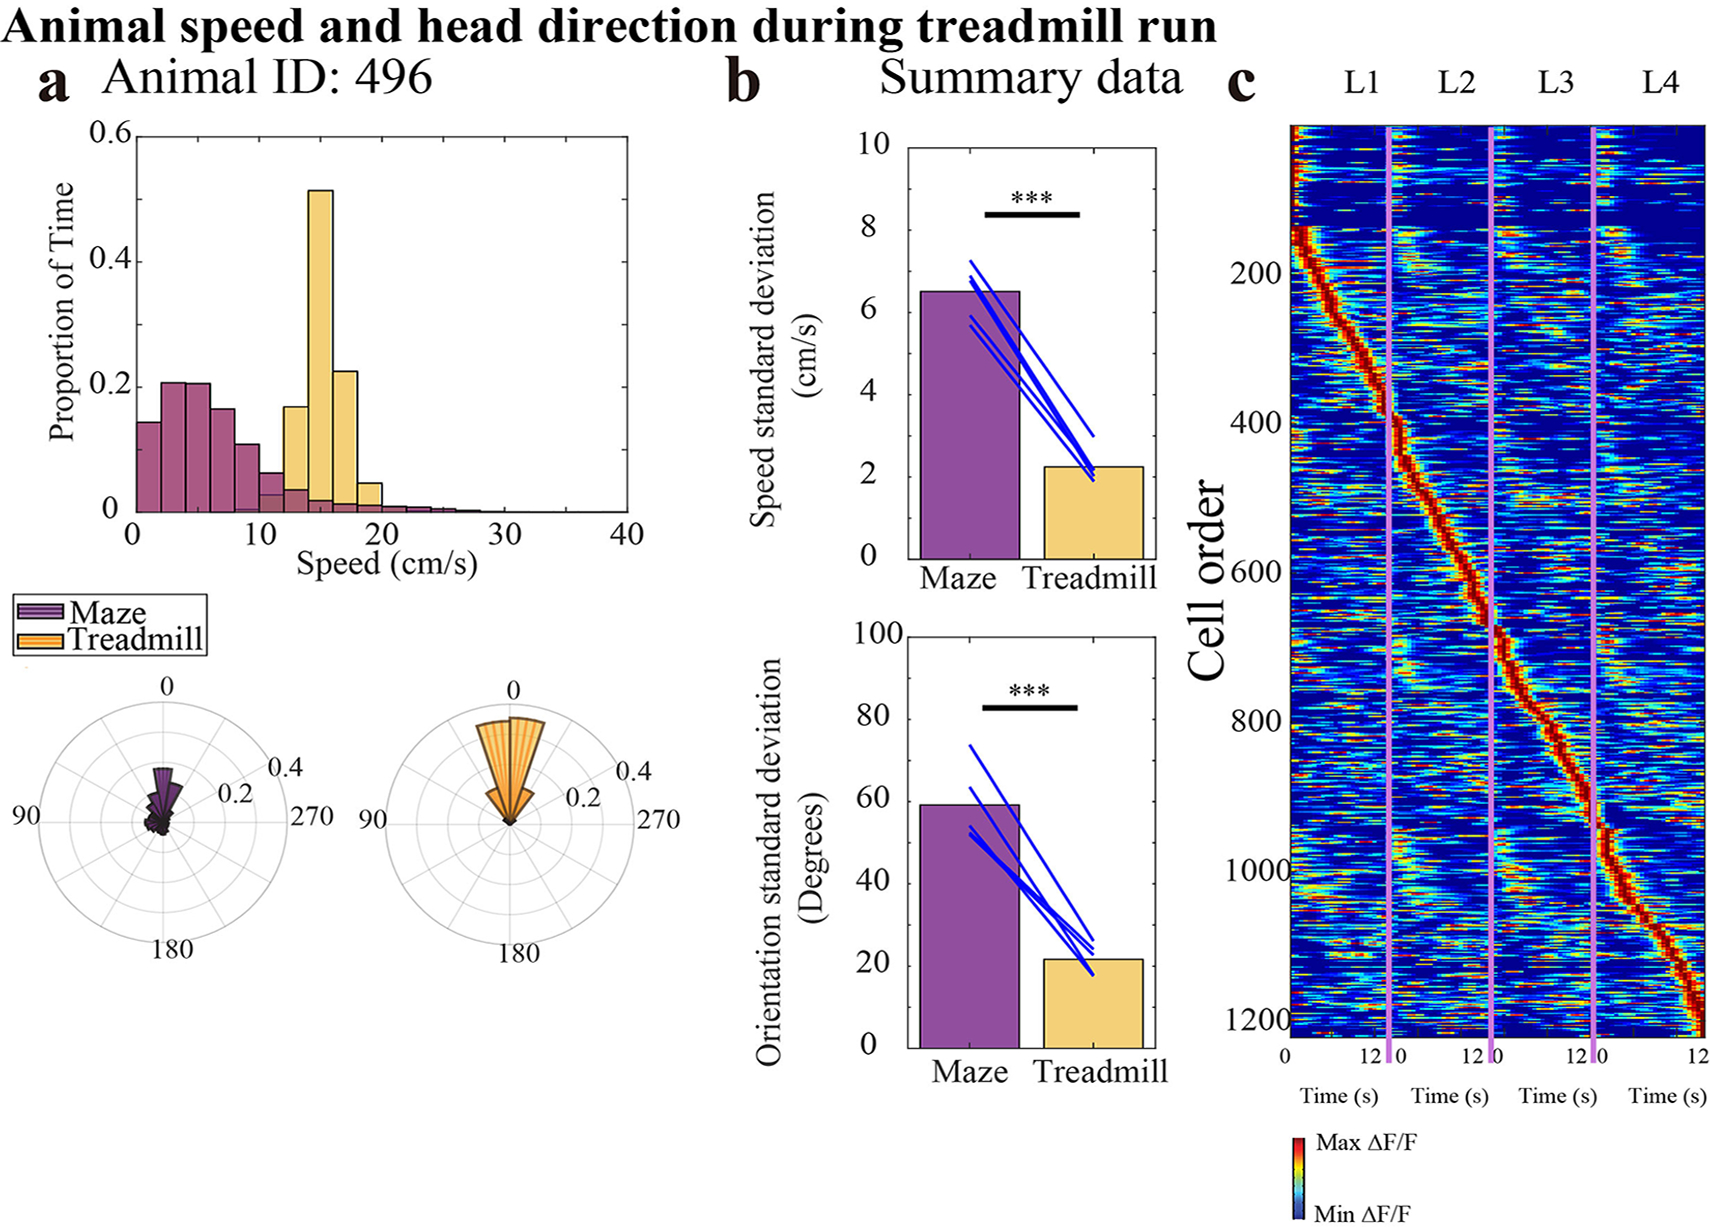
\includegraphics[width=\textwidth]{figures/ch_sun2020/extended_fig9.jpg}
\caption[Extended Data Fig.~9: Treadmill running kinematics]{\textbf{Extended Data Fig.\ 9: Treadmill running kinematics.}
(a--b) Running speed distributions and head direction changes during the treadmill period, confirming that speed and head direction were nearly constant on the treadmill. This validates the use of treadmill-period activity as a non-spatial calcium signal that does not require the linear model correction applied to maze-running data.}
\label{fig:sun2020-ext9}
\end{figure}

\begin{figure}[htbp]
\centering
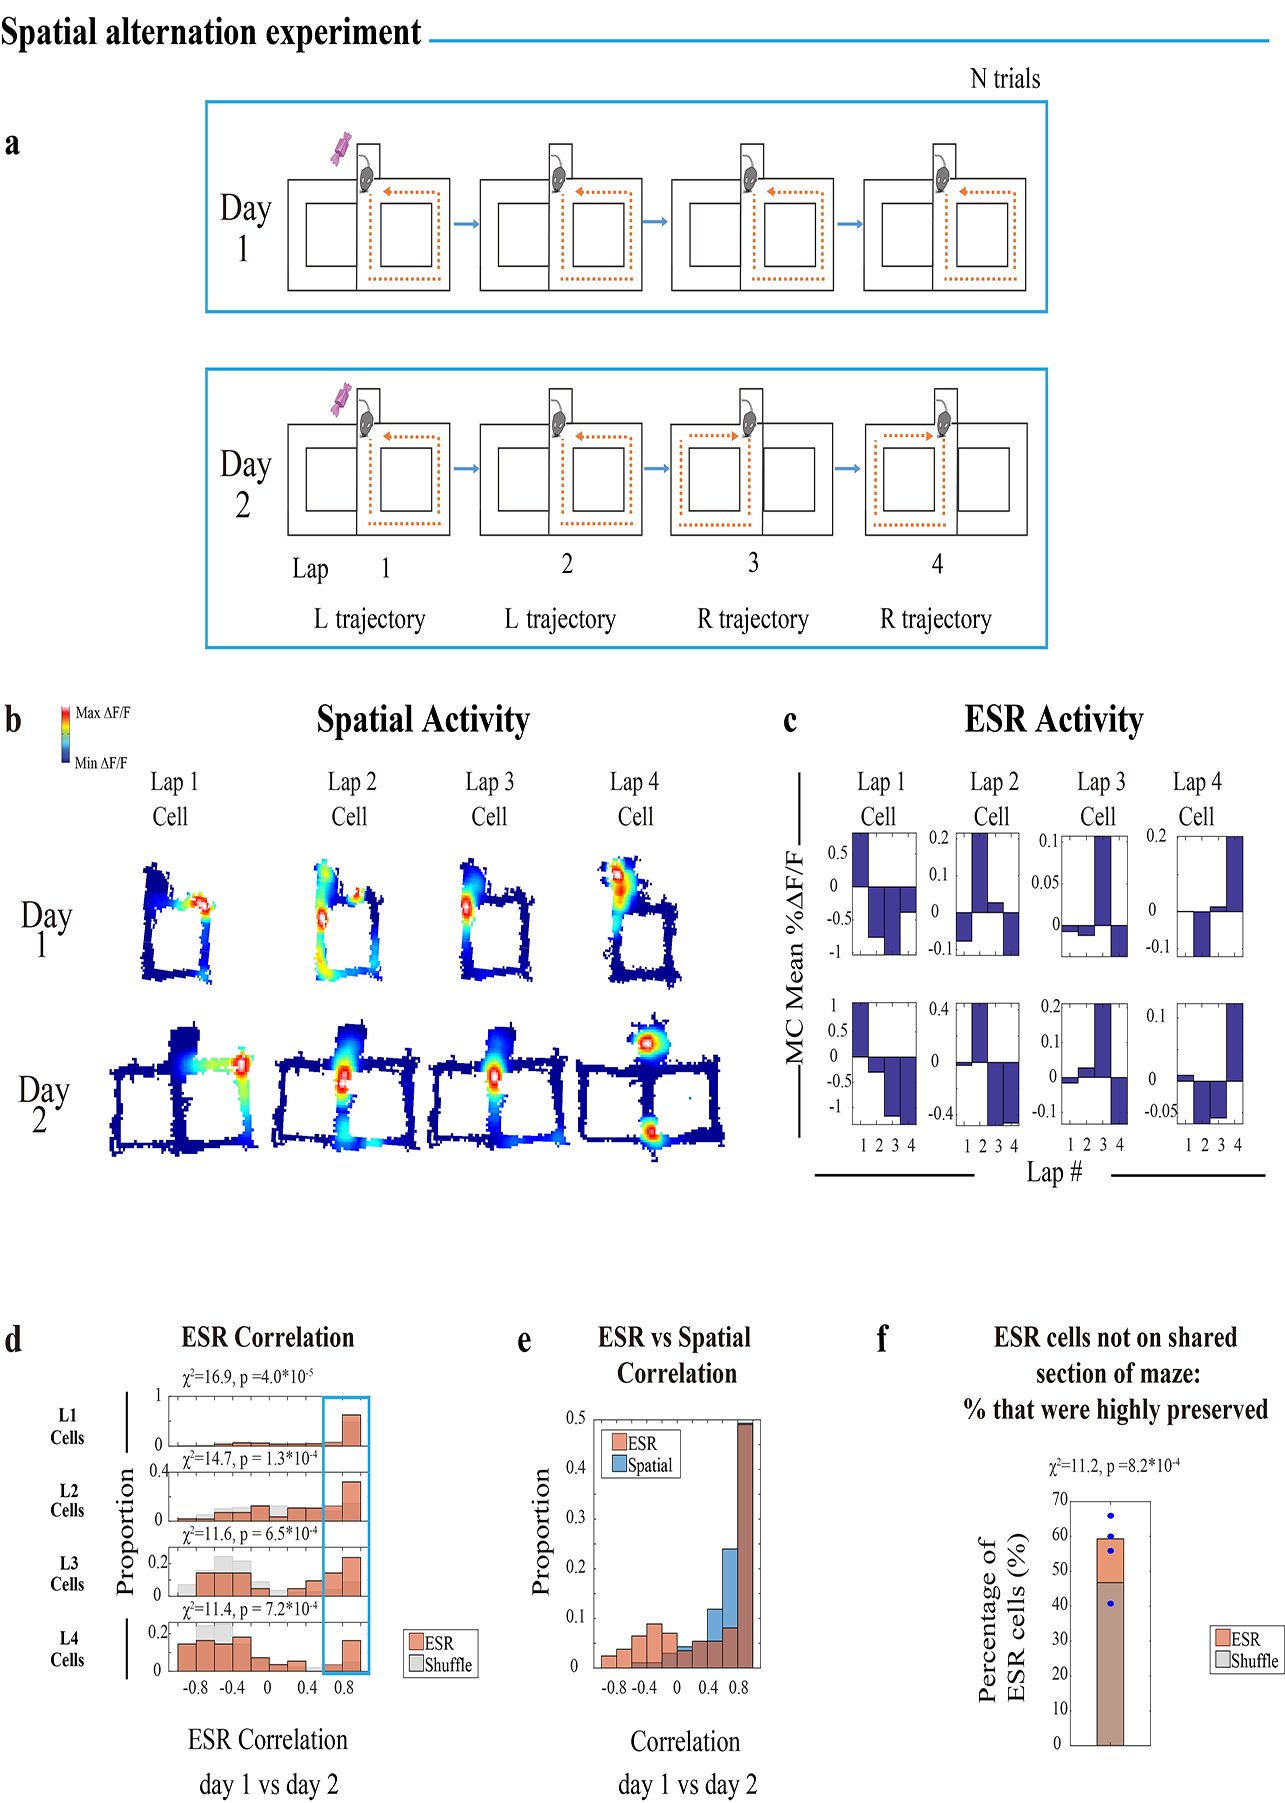
\includegraphics[width=\textwidth]{figures/ch_sun2020/extended_fig10.jpg}
\caption[Extended Data Fig.~10: Spatial alternation experiment]{\textbf{Extended Data Fig.\ 10: Spatial alternation experiment.}
(a) Spatial alternation experiment design: the spatial trajectory alternated every two laps while the 4-laps-per-reward structure was maintained.
(b--c) Behavioral data confirming that animals correctly navigated the alternating spatial trajectories.
(d) ESR correlations across the standard and spatial alternation sessions, confirming that a significant proportion of lap 1--4 ESR cells maintained their lap-specific activity patterns despite differential spatial trajectories on different laps (Extended Data Fig.\ 6e: raw $\Delta F/F$).}
\label{fig:sun2020-ext10}
\end{figure}
